\section{Historique}
\subsection{1950}
\subsection{1970}
\subsection{1980}
\begin{frame}{Historique}
    \begin{itemize}[<+-|alert@+>]
        \myitem 1950
        \myitem 1970
        \myitem à partir de 1980
        \myitem 1980
        \myitem récent
    \end{itemize}

    \only<1>{
        \vspace{-20mm}
        \begin{columns}[T,onlytextwidth]
            \column{0.75\textwidth}
            \begin{exampleblock}{Naissance du mot}
                ce concept existe depuis des décennies mais, jusqu'en 1950, les
                gens ignoraient le terme. John McCarthy, connu comme le
                fondateur de l'intelligence artificielle, a introduit le terme
                ``intelligence artificielle'' en 1950, avec l'objectif de faire
                produire des tâches humaines par des machines mimant l'activité du
                cerveau.

                %que ce soit par des algorithmes des
                %classification/reseux des neurons artificiels
                % image de alan torine dans reunis
            \end{exampleblock}
            \column{0.02\textwidth}
            \column{0.25\textwidth}
            \centering
            \vspace{10mm}
            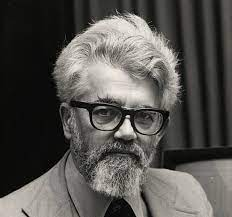
\includegraphics[height=\textwidth,width=\textwidth]{jon_maccrthy.jpg}
        \end{columns}
    }

    \only<2>{
        \vspace{-15mm}
        \begin{exampleblock} {Création des algorithmes}
            les scientifique ont pris fin à création de tous les algorithmes
            d'intelligence artificiels, mais la puissance des ordinateurs sont très
            faibles
        \end{exampleblock}
        \vspace{1mm}
        \centering
        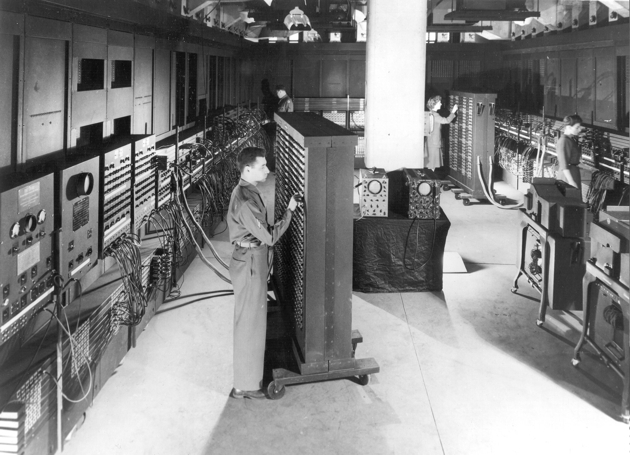
\includegraphics[height=0.4\textwidth,width=0.8\textwidth]{1970.jpg}
    }

    \only<3>{
        \vspace{-5mm}
        \begin{columns}[T,onlytextwidth]
            \column{0.75\textwidth}
            \begin{exampleblock}{Réseaux des neurones artificielle}
                développement des réseaux de neurones artificiels, grâce à l'augmentation
                de puissance des ordinateurs et à l'accumulation des gigantesques quantités
                de données(big data).
            \end{exampleblock}
            \column{0.02\textwidth}
            \column{0.25\textwidth}
            \centering
            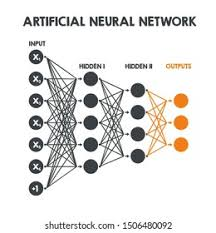
\includegraphics[height=\textwidth,width=\textwidth]{neuron.jpg}
        \end{columns}
    }
    \only<4>{
        \vspace{-10mm}
        \begin{exampleblock}{Mycin}
        le développement du premier applications qui utilise le \textbf{IA} dans le
        domaine de médecine, qui capable de reproduire les mécanismes cognitifs
        d'un expert, Les plus célèbres, Mycin (identification d'infections
        bactériennes) s'appuient sur l'ensemble des connaissances médicales
        dans un domaine donné et une formalisation des raisonnements des
        spécialistes qui lient ces connaissances entre elles pour aboutir à un
            diagnostic.
            %\cite{c1,c2,c3,c4,c5}
    \end{exampleblock}
    }

    \only<5>{
    \begin{exampleblock}{Google}
        Google AI mis au point une \textbf{IA} qui prédit le cancer du poumon avec
        $94,4~\%$ de réussite. Ces procédures permettent aussi d'éviter des
        tests invasifs comme des biopsies. L'IA apporte également une aide à
        la prescription, par exemple en détectant automatiquement un risque
        d'allergie ou d'interaction médicamenteuse.\mybox
    \end{exampleblock}
    }


    \vspace{80mm}
\end{frame}
